% Plantilla común para figuras redibujadas (fig-NN-desc.tex).
% Copiar entera y sustituir solo el cuerpo entre las marcas "cuerpo de la figura".
% Compila tal cual en Overleaf o con scripts/tikz2svg.sh.
%
% NO añadir la opción "tikz" a standalone: parte cada tikzpicture (y cada
% \chemfig) en una página distinta y el SVG solo tendría la primera.
\documentclass[border=4pt]{standalone}
\usepackage[T1]{fontenc}
\usepackage{lmodern}            % base vectorial: sin fuente vectorial el texto sale en Type 3 y dvisvgm lo pierde
\usepackage[scaled=0.95]{helvet}% sans-serif tipo Helvetica, como la interfaz de Obsidian
\renewcommand{\familydefault}{\sfdefault}
\usepackage{amsmath,amssymb}
\usepackage{sansmath}\sansmath  % fórmulas en sans, a juego con el texto
\usepackage[version=4]{mhchem}  % \ce{A + B -> C}
\usepackage{chemfig}            % estructuras y esquemas de reacción
\usepackage{tikz}
\usetikzlibrary{arrows.meta,positioning,calc,shapes.geometric,decorations.pathmorphing,decorations.markings}
\usepackage{pgfplots}           % gráficas (cinética, curvas de valoración...)
\pgfplotsset{compat=1.18}

% ---- Estilo Apuntes.md --------------------------------------------------
% Paleta semántica (la misma que el CSS de Obsidian). Principios inspirados en
% figures4papers (ChenLiu-1996, CC BY-NC 4.0): se adoptan ideas, no código.
\definecolor{apAzul}{HTML}{0F4D92}       % anotaciones, estructura (el azul del autor)
\definecolor{apAzulClaro}{HTML}{3775BA}
\definecolor{apRojo}{HTML}{B64342}       % curvas y datos principales, importante (el rojo del autor)
\definecolor{apRojoClaro}{HTML}{E9A6A1}
\definecolor{apVerde}{HTML}{3B7D3B}      % definiciones, "positivo"
\definecolor{apVerdeClaro}{HTML}{AADCA9}
\definecolor{apGris}{HTML}{767676}       % apoyo: rejillas, referencias, líneas punteadas
\definecolor{apGrisClaro}{HTML}{CFCECE}
\definecolor{apNegro}{HTML}{272727}      % ejes y texto neutro

\tikzset{
  % sin "color=" global: pisaría los \color{...} de chemfig (estructuras en rojo, etc.)
  every picture/.append style={line width=0.9pt, >={Stealth[length=2.4mm]}},
  curva/.style={apRojo, line width=1.6pt},                  % la curva o el dato que importa
  curva secundaria/.style={apAzulClaro, line width=1.3pt},
  referencia/.style={apGris, dotted, line width=1pt},       % líneas guía (p. ej. y = 0)
  anotacion/.style={apAzul, font=\normalsize},              % texto escrito a mano alrededor del dibujo
  flecha/.style={->, apAzul, line width=1pt},
  implica/.style={-{Implies}, double, double distance=2pt, line width=0.8pt},
  marca/.style={circle, fill=apAzul, draw=white, line width=0.6pt, inner sep=1.8pt},
  resalte/.style={apAzul, line width=1pt},                  % círculos/óvalos que rodean algo
}
\pgfplotsset{
  apuntes/.style={
    axis lines=left, axis line style={line width=1pt, apNegro, -{Stealth[length=2.4mm]}},
    tick style={apNegro, line width=0.8pt}, tick align=outside,
    label style={font=\normalsize}, tick label style={font=\normalsize},
    every axis plot/.append style={curva},
    clip=false,
  },
}
\setchemfig{atom sep=2em, bond style={line width=0.9pt}}
% -------------------------------------------------------------------------

\begin{document}
% --- cuerpo de la figura ---
% Forma de los lípidos -> agregado: cono invertido -> micela; cilindro -> bicapa -> vesícula
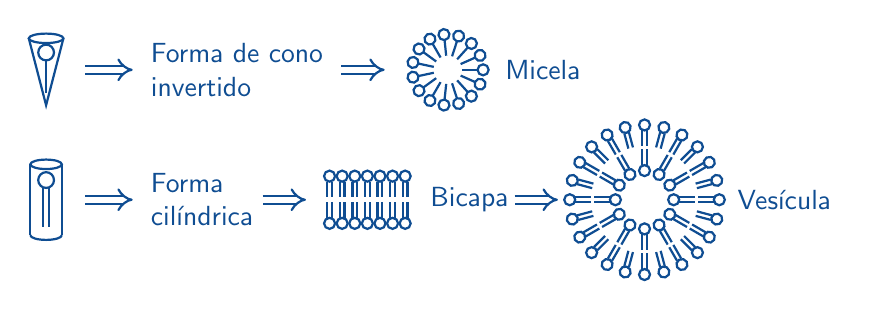
\begin{tikzpicture}[apAzul, thick, font=\normalsize,
  imp/.style={-{Implies}, double, double distance=2pt}]
  % un lípido: cabeza (círculo) en (x,y); las colas salen en la dirección opuesta a "ángulo"
  % (ángulo = hacia dónde mira la cabeza)
  \newcommand{\lipido}[4]{% x, y, ángulo de la cabeza, nº de colas (1 o 2)
    \begin{scope}[shift={({#1},{#2})}, rotate=#3]
      \draw[fill=white] (0,0) circle (0.07);
      \ifnum#4=1 \draw (-0.07,0) -- (-0.27,0);
      \else \draw (-0.07,0.03) -- (-0.27,0.03); \draw (-0.07,-0.03) -- (-0.27,-0.03); \fi
    \end{scope}}

  % ---- fila 1: cono invertido -> micela (cabezas fuera, colas dentro)
  \draw (-0.22,1.0) -- (0,0.15) -- (0.22,1.0);
  \draw (0,1.0) ellipse (0.22 and 0.06);
  \draw[fill=white] (0,0.82) circle (0.1);
  \draw (0,0.72) -- (0,0.3);
  \draw[imp] (0.5,0.6) -- (1.1,0.6);
  \node[align=left, anchor=west] at (1.2,0.6) {Forma de cono\\invertido};
  \draw[imp] (3.75,0.6) -- (4.3,0.6);
  \foreach \t in {0,24,...,359} \lipido{5.1+0.45*cos(\t)}{0.6+0.45*sin(\t)}{\t}{1};
  \node[anchor=west] at (5.7,0.6) {Micela};

  % ---- fila 2: cilindro -> bicapa -> vesícula
  \draw (-0.2,-0.6) -- (-0.2,-1.5) (0.2,-0.6) -- (0.2,-1.5);
  \draw (0,-0.6) ellipse (0.2 and 0.06);
  \draw (-0.2,-1.5) arc (180:360:0.2 and 0.06);
  \draw[fill=white] (0,-0.8) circle (0.1);
  \draw (-0.04,-0.9) -- (-0.04,-1.4) (0.04,-0.9) -- (0.04,-1.4);
  \draw[imp] (0.5,-1.05) -- (1.1,-1.05);
  \node[align=left, anchor=west] at (1.2,-1.05) {Forma\\cilíndrica};
  \draw[imp] (2.75,-1.05) -- (3.3,-1.05);
  \foreach \i in {0,...,6} {
    \lipido{3.6+0.16*\i}{-0.75}{90}{2};
    \lipido{3.6+0.16*\i}{-1.35}{-90}{2};
  }
  \node[anchor=west] at (4.75,-1.05) {Bicapa};
  \draw[imp] (5.95,-1.05) -- (6.5,-1.05);
  % vesícula: capa externa (cabezas fuera) e interna (cabezas dentro, hacia la luz)
  \foreach \t in {0,15,...,359} \lipido{7.6+0.95*cos(\t)}{-1.05+0.95*sin(\t)}{\t}{2};
  \foreach \t in {0,30,...,359} \lipido{7.6+0.37*cos(\t)}{-1.05+0.37*sin(\t)}{\t+180}{2};
  \node[anchor=west] at (8.65,-1.05) {Vesícula};
\end{tikzpicture}
% ---------------------------
\end{document}
